% Offizielle Beispieldatei für beamer-Vorlage aus tubslatex Version 0.3alpha2
\documentclass[fleqn,11pt]{beamer}

\usepackage[ngerman]{babel}
\usepackage[utf8x]{inputenc}
\usepackage{graphicx}
\usepackage{eurosym} % Für die Hardwarepreise
\usepackage{textpos}  % Für Grafikpositionierung
\usepackage{ulem}
\usetheme[%
  %cmyk,%<rgbprint>,          Auswahl des Farbmodells
  blue,%<orange/green/violet> Auswahl des Sekundärfarbklangs
  dark,%<light,medium>        Auswahl der Helligkeit
  %colorhead,%    Farbig hinterlegte Kopfleiste
  %colorfoot,%    Farbig hinterlegt Fußleiste auf Titelseite
  colorblocks,%   Blöcke Farbig hinterlegen
  %nopagenum,%    Keine Seitennumer in Fußzeile
  %nodate,%       Kein Datum in Fußleiste
  tocinheader,%   Inhaltsverzeichnis in Kopfleiste
  %tinytocinheader,% kleines Kopfleisten-Inhaltsverzeichnis
  %widetoc,%      breites Kopfleisten-Inhaltsverzeichnis
  %narrowtoc,%    schmales Kopfleisten-Inhaltsverzeichnis
  %nosubsectionsinheader,%  Keine subsections im Kopfleisten-Inhaltsverzeichnis
  %nologoinfoot,% Kein Logo im Fußbereich darstellen
  ]{tubs}

% Titelseite
\title{FAIL - Failed Accustic Indoor  Localication
(Abschlusspräsentation)}
\subtitle{Praktikum Wireless Sensor Networks - Team 4}
\author{Johannes Starosta, Lena Schimmel}
% Titelgrafik, automatisch beschnitten, Weitere Optionen: <scaled/cropx/cropy>
% \titlegraphic[cropped]{\includegraphics{infozentrum.jpg}}
\titlegraphic[scaled]{
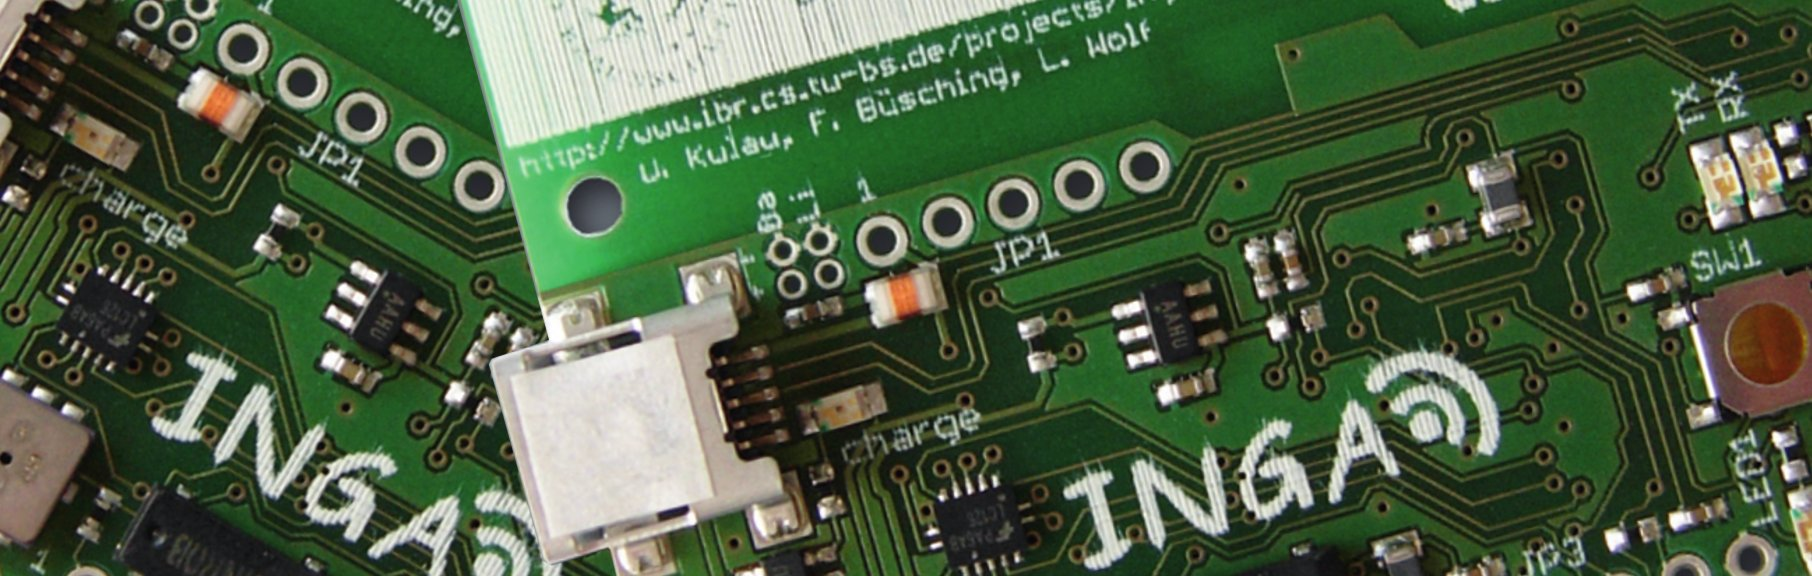
\includegraphics{titlepicture3.jpg}
\sout{AIO - Akustische Indoor-Ortung \\(Abschlusspräsentation)}
}

% Logo, dass auf Titelseiten oben rechts und auf Inthaltsseiten unten rechts
% dargestellt wird. Es wird jeweils automatisch skliert
\logo{
\includegraphics{ibr.jpg}}
%\logo{Institut für Unkreativität\\und Schreibschwäche}

\begin{document}

\begin{frame}[plain]
\titlepage
\end{frame}

\begin{frame}{Kurze Wiederholung: Idee}
	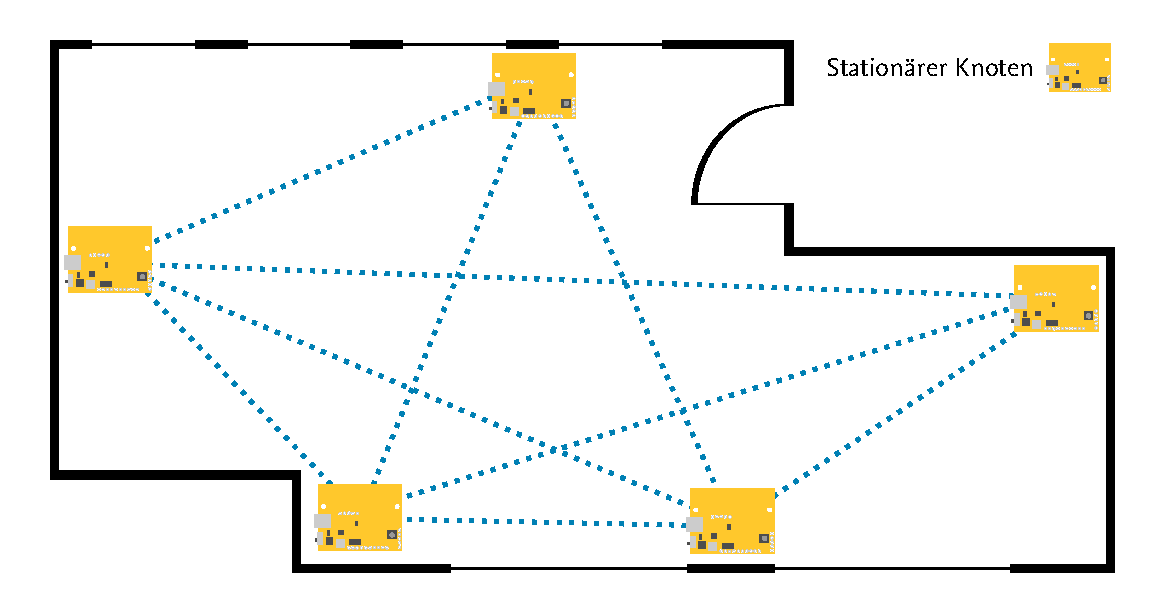
\includegraphics[width=0.48\textwidth]{room-2.pdf}
	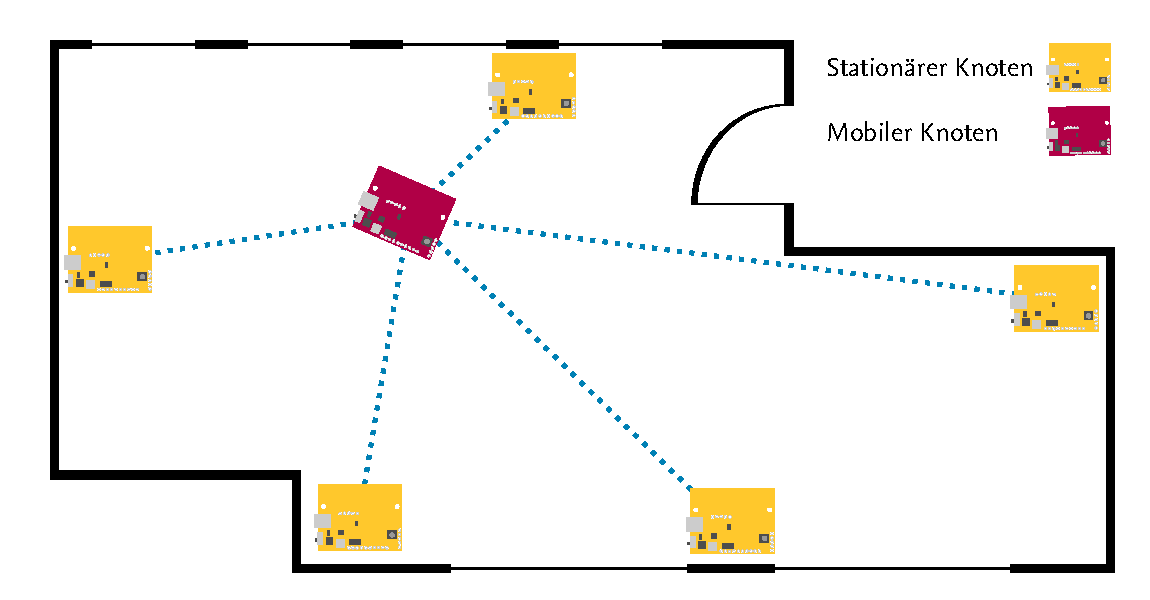
\includegraphics[width=0.48\textwidth]{room-3.pdf}
	\begin{itemize}
		\item Stationäre Knoten bestimmen ihre relative Lage zueinander
		\item Anschließend werden mobile Knoten geortet
		\item Beides geschieht über Laufzeitmessung akustischer Signale
	\end{itemize}
\end{frame}

\begin{frame}{Aktueller Status}
  \textbf{Was gehen sollte:}
	\begin{itemize}
	  \item    Hardware-Erweiterung für Audioverarbeitung
	  \item  Zeitsynchronisation im Bereich von Millisekunden
	  \item   Knoten können auf Aufforderung akkustische Signale senden
	  \item   Signale können hörbar und unhörbar (ab 18 kHz sein)
	  \item   Laufzeitmessung besagter Signale
	  \item   Lokalisierung der Knoten im Raum
	  \item   GUI zur Visualisierung

	\end{itemize}
	
	\textbf{Was tatsächlich geht:}
	\begin{itemize}
	  \item Hardware-Erweiterung für Audioverarbeitung
	  \item   Unterstützt aber nur hörbare Signale
	  \item  Zeitsynchronisation
	  \item   Laufzeitmessung
	\end{itemize}
\end{frame}

\begin{frame}{Aufgetretende Probleme: Zeitsynchronisation}

	\begin{itemize}
	  \item Knoten müssen Zeit synchron halten
	  \item  Problem: Interne Uhr startet bei 0 und läuft regelmäßig über
	    ( < 2 min, da nur 16 Bit verwendet)
	  \item  Idee: Eigenen Zähler definieren, der bei Überlauf hoch
	    zählt,
	    daraus 32-Bit-Zeit ableiten
	  \item  Knoten blockieren sich gegenseitig (Deadlocks)
	   \item Interne Uhr läuft unterschiedlich schnell (je nach INGA
	    langsamer
	    oder schneller)
	   \item Fehlerbehebung langwierig
	    \item Geht jetzt aber :)
	\end{itemize}
\end{frame}


\begin{frame}{Zeitsynchronisation: Umsetzung}
	\begin{itemize}
	    \item Definition eines Paketformates (wird auch an anderer Stelle
	    benötigt) zum Austausch von Informationen zur Zeit und zum
	    Betriebsmodus
	  \item Erwähnter Zähler definiert lokale Uhr
	  \item    Ein Master-Knoten dient als Referenz für den Rest
	  \item  Im Sekundentakt fragen die Slaves dem Master den Master ab
	  \item   Aus Rücklaufzeit der Antwort und Offeset der lokalen Zeit
	    gegenüber Referenzzeit bestimmen die Slaves die ,,Echtzeit''

	\end{itemize}
\end{frame}

\begin{frame}{Aufgetretende Probleme: Audio-Erweiterung}
	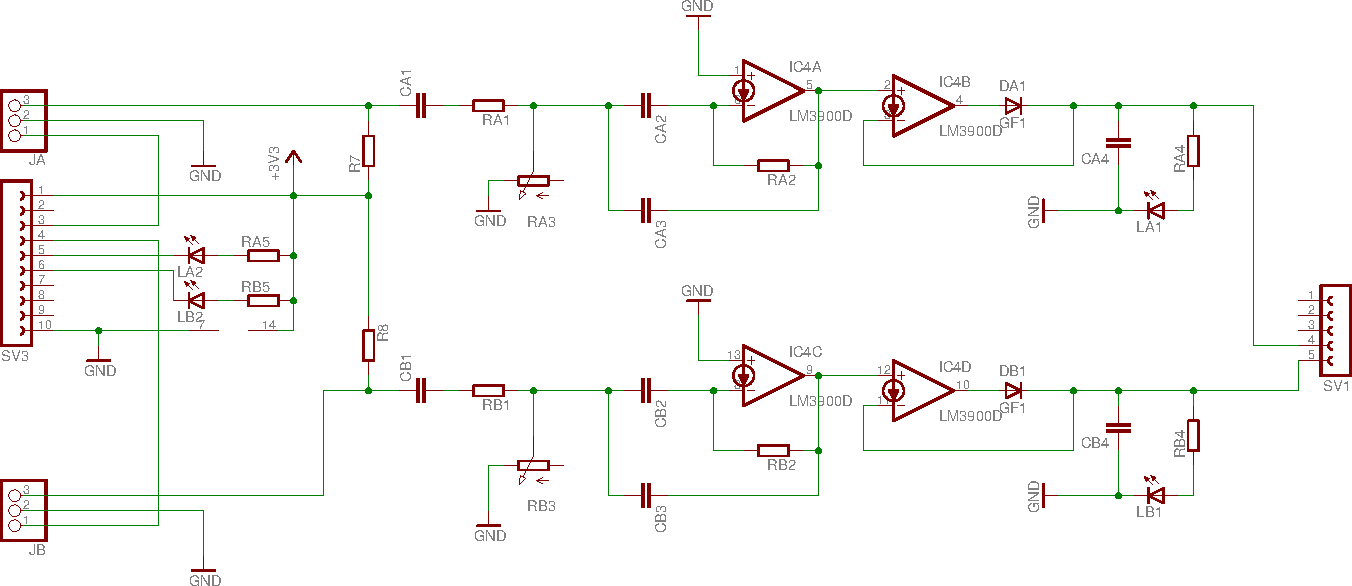
\includegraphics[width=0.9\textwidth]{AudioBoardSchema.pdf}
	\begin{itemize}
	  \item ,,Naiver Ansatz"`: Bestehendes Schaltbild nehmen und
	    anpassen
	   \item
	    Angedachte Funktionen:
	    \begin{itemize}
	      \item    Audio-Eingabe, Vorverstärker und Bandpassfilter (Aufnahme
	       und	          Sampling)
	     \item   Audio-Ausgabe: Verstärker und Lautsprecher
	\end{itemize}
	\end{itemize}
\end{frame}

\begin{frame}{Aufgetretende Probleme: Audio-Erweiterung}
	\begin{itemize}
	  \item  Schaltung funktionierte nicht wie vorgesehen
	  \item   Analoger Filter produzierte Datenmüll (cool für
	       Zufallsgenatoren!)
	     \item   Digitaler Bandpassfilter (in Software): Relativ
		  geringe Wirkung im
		     Verhältnis zum Aufwand, ihn weglassen hat nichts
		     verschlechtert!
		   \item	        Audioverarbeitung erfolgt jetzt rein in Software
		   \item   Pezzo-Lautsprecher hatten nicht genug Power
			   mit unserer Schaltung
			 \item 	      Lösung: Lautsprecher
			   (,,Signalgeber'' von Conrad) mit interner Fertiglösung
			 \item  Funktioniert, kann aber nur mit
				 6,5 kHz ausgeben (*pieeeeeps*)
			       \item	    Höhere Frequenzen kann  Microcontroller nicht samplen

	\end{itemize}
\end{frame}

\begin{frame}{Provisorische Audio-Erweiterung}
	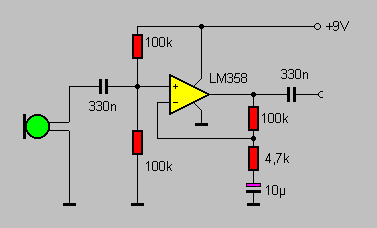
\includegraphics[width=0.5\textwidth]{opvmikro}
	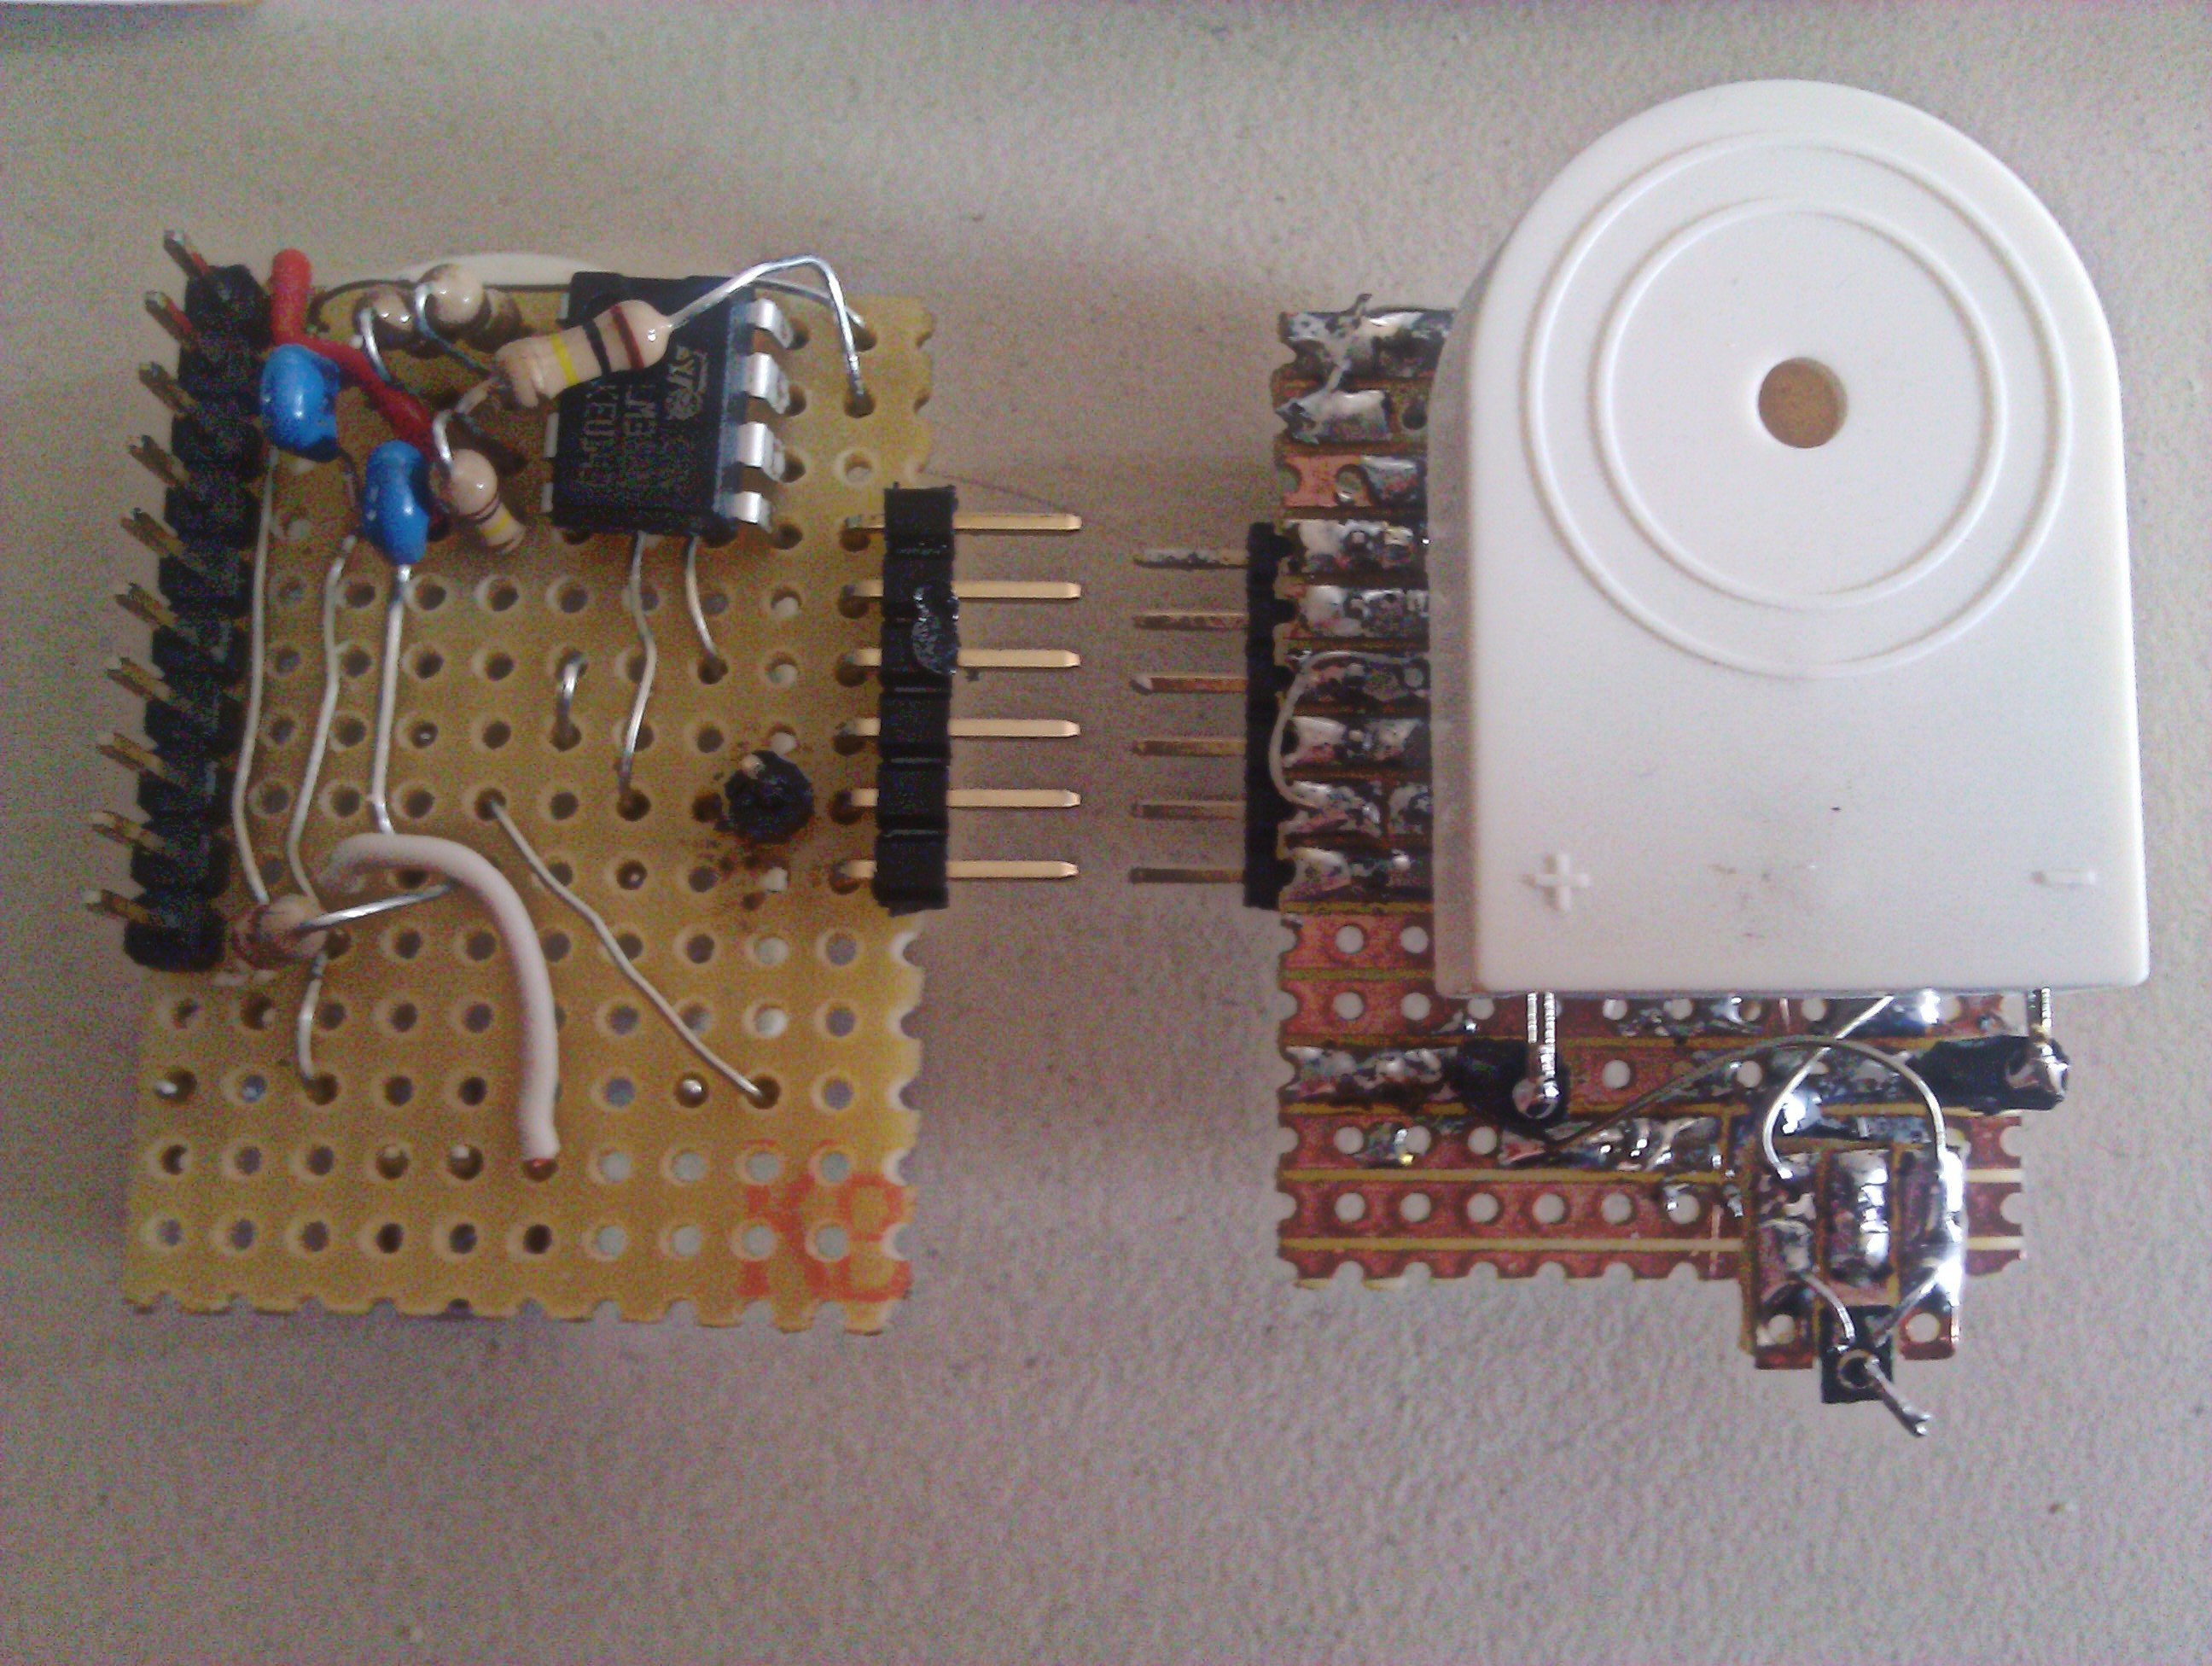
\includegraphics[width=0.5\textwidth]{two_boards_op}
      \end{frame}

      \begin{frame}{Was noch zu retten war}
	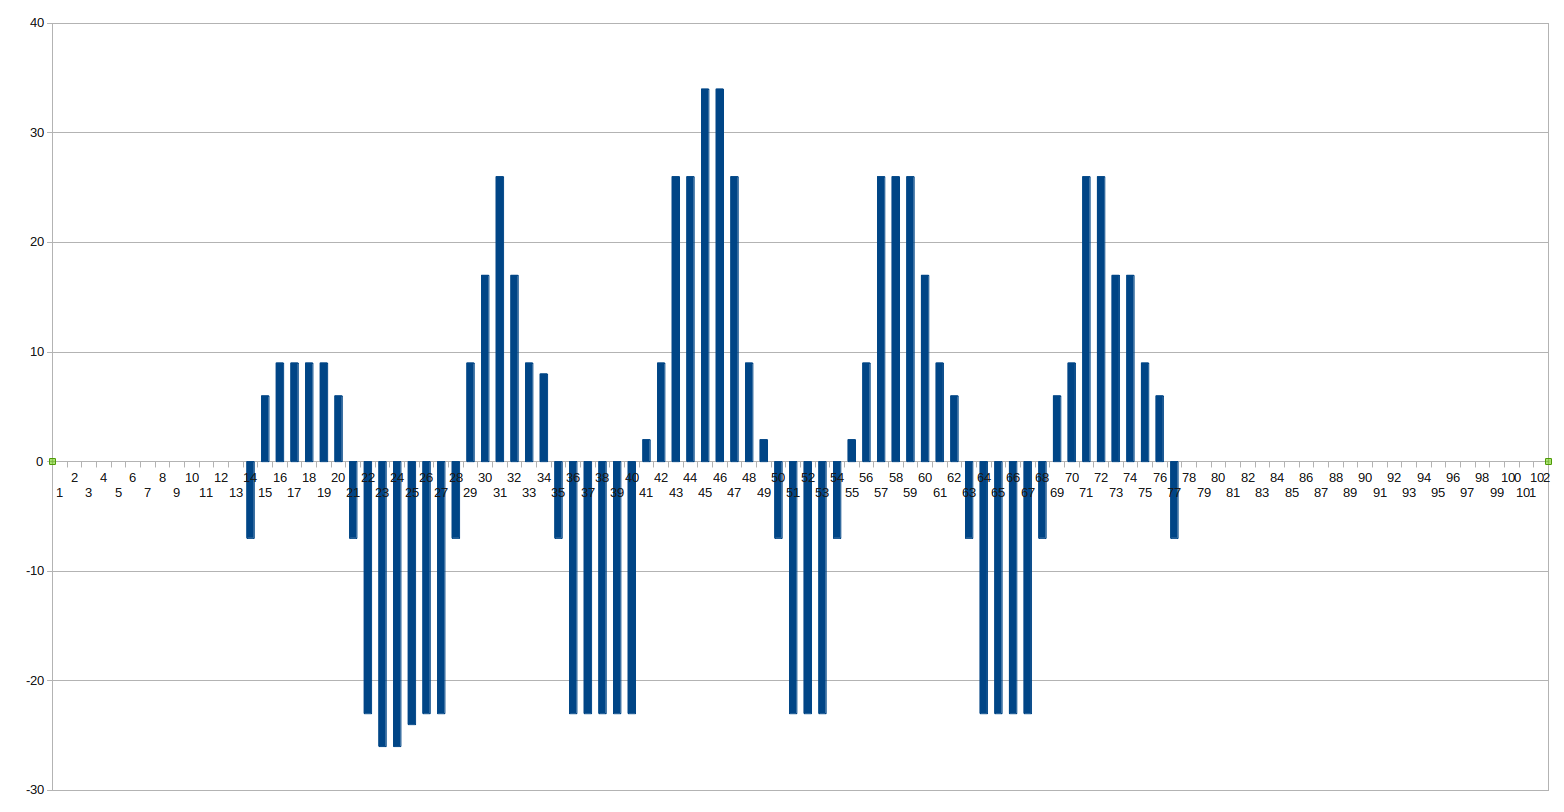
\includegraphics[width=\textwidth]{wave}
      \end{frame}


      \begin{frame}{Was noch zu retten war}
	\begin{itemize}
	  \item	    Fazit: Hardware-Erweiterung mehr oder weniger fehlgeschlagen
	  \item Bestehende Workarounds taugen nur als Proof of Concept
	  \item   Erst spät fertig geworden (letzte Woche), dadurch nur
	           begrenzte  Zeit für eigentliche Software
		 \item Was kann \sout{AIO} FAIL aktuell?
		   \begin{itemize}
		     \item 	       Signalplanung
	          \item  Aufzeichnung und Verarbeitung der Signale
		  \item   Laufzeitenmessung auf Basis der Signalwerte
		        ,,Visualisierung"` in ASCII-Modus :)

	\end{itemize}
	\end{itemize}
      \end{frame}


      \begin{frame}{Weiterführende Arbeiten}
	\begin{itemize}
      \item Lokalisierung im Raum mit bestehenden Workarounds
	implementieren
      \item Vernünftige Hardwareerweiterung implementieren, die die
	Schwächen unseres aktuellen Ansatzes vermeidet
      \item Zeitsynchronisation in Contiki integrieren
      \item Diverse Nice-To-Haves aus unserer Wikiseite
    \end{itemize}
      \end{frame}
      \begin{frame}
	\begin{itemize} \Large
	  \item Live-Demo
	  \item Fragen
	  \item \url{https://github.com/johannesst/aio-wsn/}
	\end{itemize}
      \end{frame}
      \begin{frame}
	\begin{center}
	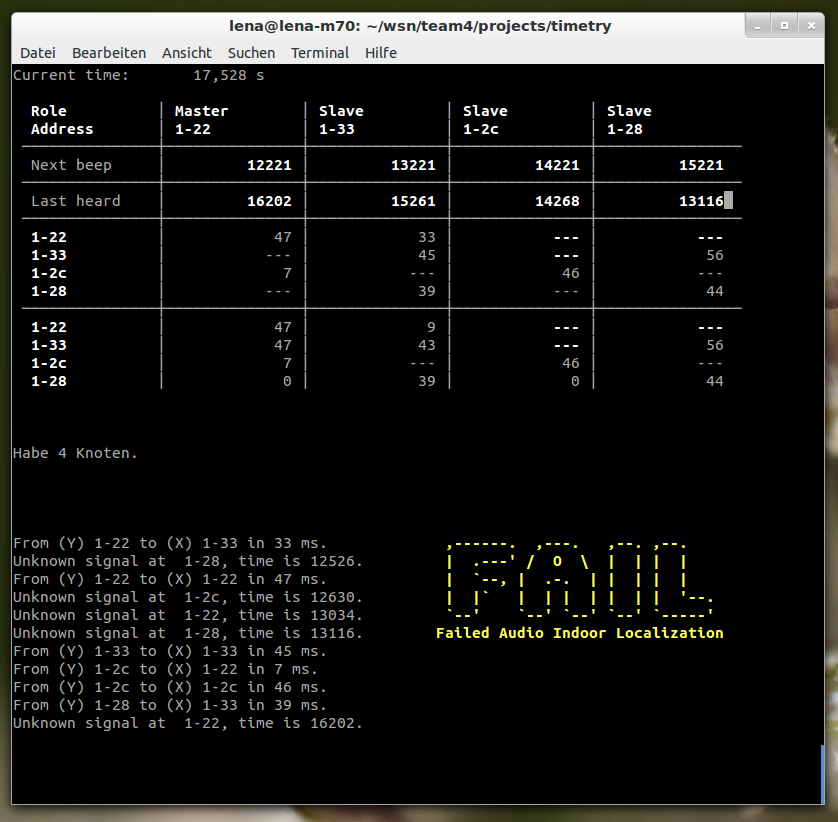
\includegraphics[width=0.7\textwidth]{screenshot}
      \end{center}
      \end{frame}
\end{document}
